\begin{figure}[htbp]
    \centering
    % 根据页面宽度自动缩放，保证不超页边距
    \resizebox{\textwidth}{!}{
    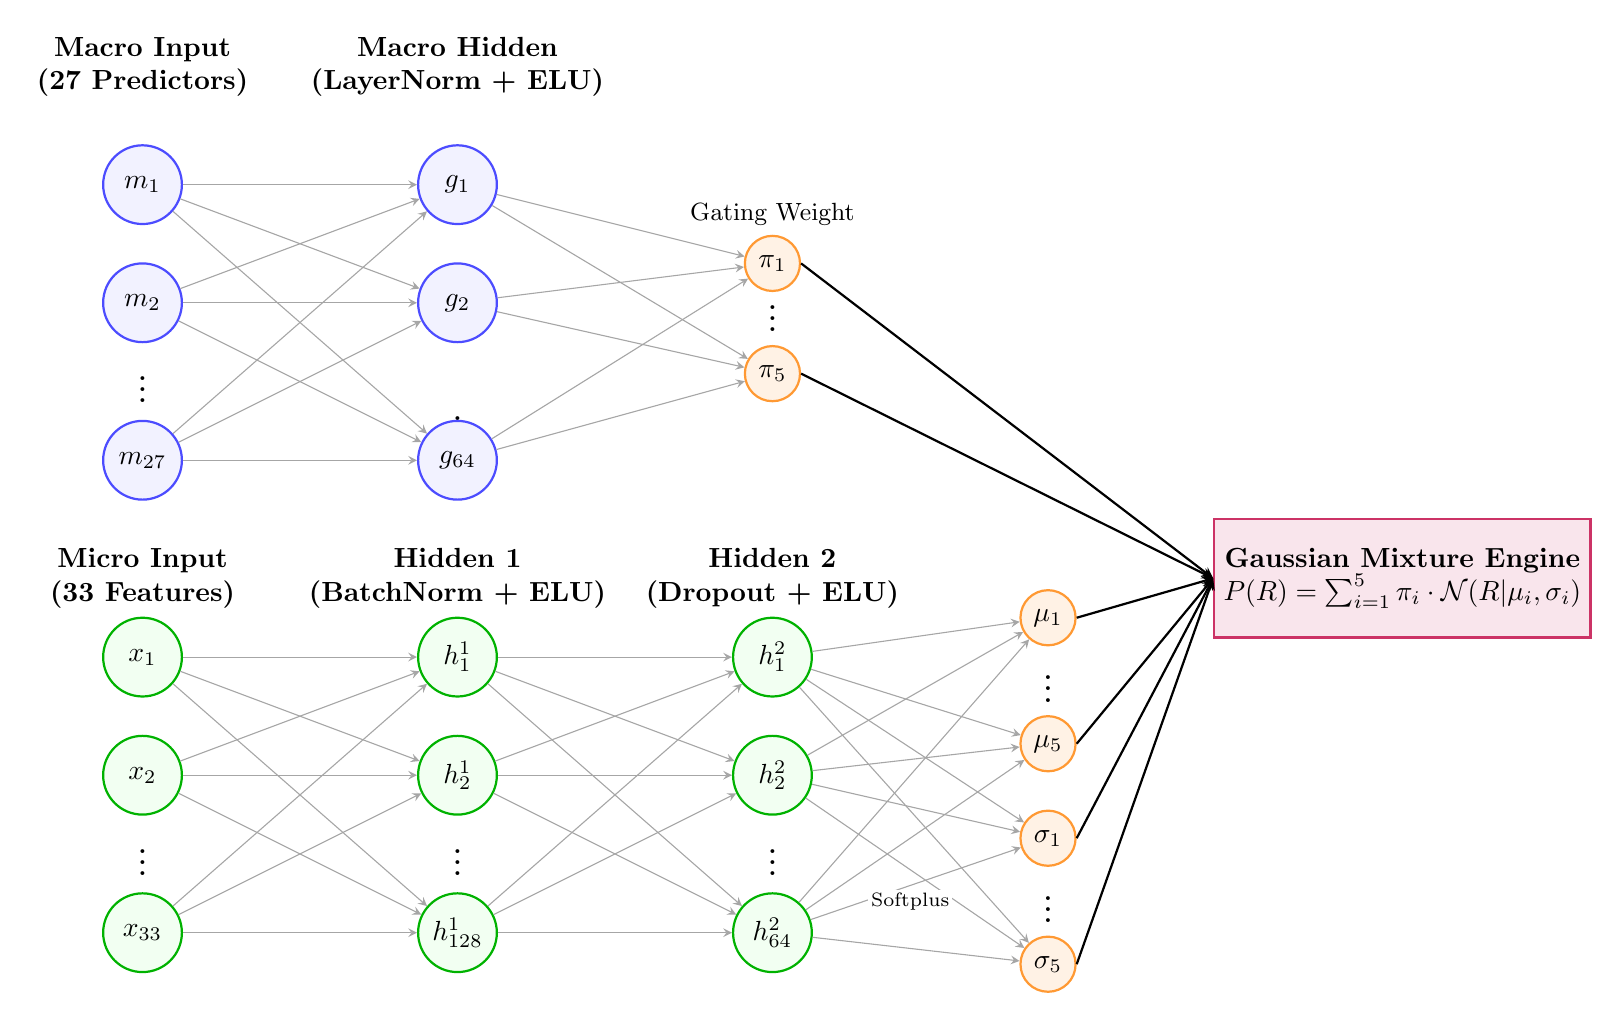
\begin{tikzpicture}[
        >=stealth, % 锐利的箭头
        macronode/.style={circle, draw=blue!70, fill=blue!5, thick, minimum size=10mm, inner sep=0pt},
        micronode/.style={circle, draw=green!70!black, fill=green!5, thick, minimum size=10mm, inner sep=0pt},
        paramnode/.style={circle, draw=orange!80, fill=orange!10, thick, minimum size=7mm, inner sep=0pt},
        engine/.style={rectangle, draw=purple!80, fill=purple!10, thick, minimum width=4cm, minimum height=1.5cm, align=center},
        output/.style={rectangle, draw=red!80, fill=red!10, thick, dashed, minimum width=4cm, minimum height=1.5cm, align=center},
        connect/.style={draw, ->, gray!70, thin}
    ]

    % ==========================================
    % 1. Macro Tower (Top Half)
    % ==========================================
    % 宏观输入层 (x=0)
    \node[macronode] (m1) at (0, 13) {$m_1$};
    \node[macronode] (m2) at (0, 11.5) {$m_2$};
    \node at (0, 10.5) {\Large $\vdots$};
    \node[macronode] (m27) at (0, 9.5) {$m_{27}$};
    \node[align=center, font=\bfseries] at (0, 14.5) {Macro Input\\(27 Predictors)};

    % 宏观隐藏层 (x=4)
    \node[macronode] (g1) at (4, 13) {$g_1$};
    \node[macronode] (g2) at (4, 11.5) {$g_2$};
    \node at (4, 10) {\Large $\vdots$};
    \node[macronode] (g64) at (4, 9.5) {$g_{64}$};
    \node[align=center, font=\bfseries] at (4, 14.5) {Macro Hidden\\(LayerNorm + ELU)};

    % 门控权重 (x=8)
    \node[paramnode] (pi1) at (8, 12) {$\pi_1$};
    \node at (8, 11.4) {\Large $\vdots$};
    \node[paramnode] (pi5) at (8, 10.6) {$\pi_5$};
    \node[above, font=\small] at (pi1.north) {Gating Weight};
    
    % 宏观直线连线 (绝对笔直)
    \foreach \i in {m1, m2, m27} {
        \foreach \j in {g1, g2, g64} {
            \path[connect] (\i) -- (\j);
        }
    }
    \path[connect] (g1) -- (pi1);
    \path[connect] (g2) -- (pi1);
    \path[connect] (g64) -- (pi1);
    \path[connect] (g1) -- (pi5);
    \path[connect] (g2) -- (pi5);
    \path[connect] (g64) -- (pi5);

    % ==========================================
    % 2. Micro Tower (Bottom Half)
    % ==========================================
    % 微观输入层 (x=0)
    \node[micronode] (x1) at (0, 7) {$x_1$};
    \node[micronode] (x2) at (0, 5.5) {$x_2$};
    \node at (0, 4.5) {\Large $\vdots$};
    \node[micronode] (x33) at (0, 3.5) {$x_{33}$};
    \node[align=center, font=\bfseries] at (0, 8) {Micro Input\\(33 Features)};

    % 隐藏层 1 (x=4)
    \node[micronode] (h1_1) at (4, 7) {$h^1_1$};
    \node[micronode] (h1_2) at (4, 5.5) {$h^1_2$};
    \node at (4, 4.5) {\Large $\vdots$};
    \node[micronode] (h1_128) at (4, 3.5) {$h^1_{128}$};
    \node[align=center, font=\bfseries] at (4, 8) {Hidden 1\\(BatchNorm + ELU)};

    % 隐藏层 2 (x=8)
    \node[micronode] (h2_1) at (8, 7) {$h^2_1$};
    \node[micronode] (h2_2) at (8, 5.5) {$h^2_2$};
    \node at (8, 4.5) {\Large $\vdots$};
    \node[micronode] (h2_64) at (8, 3.5) {$h^2_{64}$};
    \node[align=center, font=\bfseries] at (8, 8) {Hidden 2\\(Dropout + ELU)};

    % 分布参数 (x=11.5) - 重新调整了 Y 坐标以保持垂直居中
    \node[paramnode] (mu1) at (11.5, 7.5) {$\mu_1$};
    \node at (11.5, 6.7) {\Large $\vdots$};
    \node[paramnode] (mu5) at (11.5, 5.9) {$\mu_5$};
    \node[paramnode] (sigma1) at (11.5, 4.7) {$\sigma_1$};
    \node at (11.5, 3.9) {\Large $\vdots$};
    \node[paramnode] (sigma5) at (11.5, 3.1) {$\sigma_5$};

    % 微观直线连线 (绝对笔直)
    \foreach \i in {x1, x2, x33} {
        \foreach \j in {h1_1, h1_2, h1_128} {
            \path[connect] (\i) -- (\j);
        }
    }
    \foreach \i in {h1_1, h1_2, h1_128} {
        \foreach \j in {h2_1, h2_2, h2_64} {
            \path[connect] (\i) -- (\j);
        }
    }
    \foreach \i in {h2_1, h2_2, h2_64} {
        \path[connect] (\i) -- (mu1);
        \path[connect] (\i) -- (mu5);
        \path[connect] (\i) -- (sigma1);
        \path[connect] (\i) -- (sigma5);
    }
    
    % 在线上加上激活函数标注 (位置同步下移对齐 sigma)
    \node[fill=white, inner sep=1pt, font=\scriptsize] at (9.75, 3.9) {Softplus};

    % ==========================================
    % 3. Mixture Engine & Output (Far Right)
    % ==========================================
    \node[engine] (mix) at (16, 8) {\textbf{Gaussian Mixture Engine} \\ $P(R) = \sum_{i=1}^5 \pi_i \cdot \mathcal{N}(R | \mu_i, \sigma_i)$};

    % 连接到引擎 (实线加粗)
    \path[draw, ->, black, thick] (pi1.east) -- (mix.west);
    \path[draw, ->, black, thick] (pi5.east) -- (mix.west);
    \path[draw, ->, black, thick] (mu1.east) -- (mix.west);
    \path[draw, ->, black, thick] (mu5.east) -- (mix.west);
    \path[draw, ->, black, thick] (sigma1.east) -- (mix.west);
    \path[draw, ->, black, thick] (sigma5.east) -- (mix.west);
    
    \end{tikzpicture}
    }
    \caption{Architecture of the Structured Gaussian Mixture Density Network}
    \label{fig:fig_MDN_N}
\end{figure}